\title{Monografia - Janderson}

\documentclass[
	% -- opções da classe memoir --
	12pt,				% tamanho da fonte
    oneside,			% Tipo de impressão, frente-verso(twoside) ou apenas frente(oneside)
	a4paper,			% tamanho do papel. 
	% -- opções da classe abntex2 --
	chapter=TITLE,		% títulos de capítulos convertidos em letras maiúsculas
	% -- opções do pacote babel --    
	english,			% idioma adicional para hifenização
	brazil				% o último idioma é o principal do documento    
	]{abntex2}
    
    %\renewcommand{\ABNTEXpartfontsize}{\normalsize}
	%\renewcommand{\ABNTEXchapterfontsize}{ \large}
	%\renewcommand{\ABNTEXsectionfontsize}{\normalsize}
	%\renewcommand{\ABNTEXsubsectionfontsize}{\normalsize}

% ---
% Pacotes básicos 
% ---
\usepackage{lmodern}			% Usa a fonte Latin Modern			
\usepackage[T1]{fontenc}		% Selecao de codigos de fonte.
\usepackage[utf8]{inputenc}		% Codificacao do documento (conversão automática dos acentos)
\usepackage{lastpage}			% Usado pela Ficha catalográfica
\usepackage{indentfirst}		% Indenta o primeiro parágrafo de cada seção.
\usepackage{color}				% Controle das cores
\usepackage{graphicx}			% Inclusão de gráficos
\usepackage{microtype} 			% para melhorias de justificação
\usepackage{todonotes}
\usepackage{tabularx}


\definecolor{algColor}{RGB}{255,206,206} % rgb(255, 206, 206)

% Pacotes para algoritmos/pseudo-código
\usepackage{listings}

\renewcommand{\lstlistingname}{Programa}

\lstset
{ %Formatting for code in appendix
    language=C,
    basicstyle=\footnotesize,
    numbers=left,
    stepnumber=1,
    frame = single,
    showstringspaces=false,
    tabsize=2,
    breaklines=true,
    xleftmargin=10pt,
    breakatwhitespace=false,
    extendedchars=true,
    literate={á}{{\'a}}1 
             {ã}{{\~a}}1
             {é}{{\'e}}1
             {í}{{\'i}}1
             {õ}{{\~o}}1
             {ç}{{\c{c}}}1,
}

\renewcommand{\lstlistlistingname}{Lista de códigos}

% Configura a ``Lista de Códigos'' conforme as regras da ABNT (para abnTeX2)
\begingroup\makeatletter
\let\newcounter\@gobble\let\setcounter\@gobbletwo
  \globaldefs\@ne \let\c@loldepth\@ne
  \newlistof{listings}{lol}{\lstlistlistingname}
  \newlistentry{lstlisting}{lol}{0}
\endgroup

\renewcommand{\cftlstlistingaftersnum}{\hfill--\hfill}

\let\oldlstlistoflistings\lstlistoflistings
\renewcommand{\lstlistoflistings}{%
   \begingroup%
   \let\oldnumberline\numberline%
   \renewcommand{\numberline}{\lstlistingname\space\oldnumberline}%
   \oldlstlistoflistings%
   \endgroup}
% ---
% Pacotes adicionais, usados apenas no âmbito do Modelo Canônico do abnteX2
% ---
\usepackage{lipsum}				% para geração de dummy text
% ---


% ---
% Pacotes de citações
% ---
%\usepackage[brazilian,hyperpageref]{backref}	 % Paginas com as citações na bibl
\usepackage[alf, abnt-etal-cite=2]{abntex2cite}	% Citações padrão ABNT

% --- 
% CONFIGURAÇÕES DE PACOTES
% --- 

\usepackage{abntex_ufrr_dcc}


% PACOTES DE ALGORITMO

\usepackage{algpseudocode,algorithm}
% Declaracoes em Português

\algrenewcommand\algorithmicend{\textbf{FIM}}
\algrenewcommand\algorithmicdo{\textbf{FAÇA}}
\algrenewcommand\algorithmicwhile{\textbf{ENQUANTO}}
\algrenewcommand\algorithmicfor{\textbf{PARA}}
\algrenewcommand\algorithmicforall{\textbf{PARA TODO}}
\algrenewcommand\algorithmicif{\textbf{SE}}
\algrenewcommand\algorithmicthen{\textbf{ENTÃO}}
\algrenewcommand\algorithmicelse{\textbf{SENÃO}}
\algrenewcommand\algorithmicreturn{\textbf{RETORNE}}
\algrenewcommand\algorithmicfunction{\textbf{FUNÇÃO}}
% New definitions
\algnewcommand\algorithmicswitch{\textbf{ESCOLHA}}
\algnewcommand\algorithmiccase{\textbf{CASO}}
\algnewcommand\algorithmicassert{\texttt{assert}}
\algnewcommand\Assert[1]{\State \algorithmicassert(#1)}%
% New "environments"
\algdef{SE}[SWITCH]{Switch}{EndSwitch}[1]{\algorithmicswitch\ #1\ \algorithmicdo}{\algorithmicend\ \algorithmicswitch}%
\algdef{SE}[CASE]{Case}{EndCase}[1]{\algorithmiccase\ #1}{\algorithmicend\ \algorithmiccase}%
\algtext*{EndSwitch}%
\algtext*{EndCase}%


% Rearranja os finais de cada estrutura
\algrenewtext{EndWhile}{\algorithmicend\ \algorithmicwhile}
\algrenewtext{EndFor}{\algorithmicend\ \algorithmicfor}
\algrenewtext{EndIf}{\algorithmicend\ \algorithmicif}
\algrenewtext{EndFunction}{\algorithmicend\ \algorithmicfunction}

% O comando For, a seguir, retorna 'para #1 -- #2 até #3 faça'
\algnewcommand\algorithmicto{\textbf{até}}
\algrenewtext{For}[3]%
{\algorithmicfor\ #1 $\gets$ #2 \algorithmicto\ #3 \algorithmicdo}


% ---
% Configurações do pacote backref
% Usado sem a opção hyperpageref de backref
%\renewcommand{\backrefpagesname}{Citado na(s) página(s):~}
% Texto padrão antes do número das páginas
%\renewcommand{\backref}{}
% Define os textos da citação
%\renewcommand*{\backrefalt}[4]{
%	\ifcase #1 %
%		Nenhuma citação no texto.%
%	\or
%		Citado na página #2.%
%	\else
%		Citado #1 vezes nas páginas #2.%
%	\fi}%
% ---

% ---
% Informações de dados para CAPA e FOLHA DE ROSTO
% ---
\titulo{Aplicação da técnica de ávore de decisão para avaliar os dados socioeconômicos dos candidatos do vestibular da UFRR de 2018 para prever o seu desempenho}

\autor{JANDERSON ALMEIDA DOS SANTOS}
\local{Boa Vista - RR}
\data{2018}
\orientador{Delfa Mercedes Huatuco Zuasnabar}

\tipotrabalho{Monografia}

\preambulo{Monografia de Graduação apresentada ao Departamento de Ciência da Computação da Universidade Federal de Roraima como requisito parcial para a obtenção do grau de Bacharel em Ciência da Computação.}

%Trabalho de conclusão de curso  na área de Verificação de Software desenvolvido na UFRR com o %objetivo \textcolor{red}{VERIFICAR O PADRÃO DOS OUTROS TCC} de gerar casos de teste para %sistemas embarcados críticos	

% ---

%-- Informações de dado para a FOLHA DE APROVAÇÃO
\renewcommand{\dataDefesa}{01 de Fevereiro de 2017}
\renewcommand{\orientadorBanca}{Prof. MSc.Delfa Mercedes Huatuco Zuasnabar}
\renewcommand{\primeiroMembroBanca}{Prof. MSc. Miguel Raymundo Flores Santibañez}
\renewcommand{\segundoMembroBanca}{Prof. MSc. Acauan Cardoso Ribeiro}

% ---
% Configurações de aparência do PDF final

% alterando o aspecto da cor azul
\definecolor{blue}{RGB}{41,5,195}

% informações do PDF
\makeatletter
\hypersetup{
     	%pagebackref=true,
		pdftitle={\@title}, 
		pdfauthor={\@author},
    	pdfsubject={\imprimirpreambulo},
	    pdfcreator={LaTeX with abnTeX2},
		pdfkeywords={abnt}{latex}{abntex}{abntex2}{trabalho acadêmico}, 
		colorlinks=true,       		% false: boxed links; true: colored links
    	linkcolor=blue,          	% color of internal links
    	citecolor=blue,        		% color of links to bibliography
    	filecolor=magenta,      	% color of file links
		urlcolor=blue,
		bookmarksdepth=4
}
\makeatother
% --- 

% --- 
% Espaçamentos entre linhas e parágrafos 
% --- 

% O tamanho do parágrafo é dado por:
\setlength{\parindent}{1.3cm}

% Controle do espaçamento entre um parágrafo e outro:
\setlength{\parskip}{0.2cm}  % tente também \onelineskip

% ---
% compila o indice
% ---
\makeindex
% ---

% ----
% Início do documento
% ----
\begin{document}

% Retira espaço extra obsoleto entre as frases.
\frenchspacing 

% ----------------------------------------------------------
% ELEMENTOS PRÉ-TEXTUAIS
% ----------------------------------------------------------
% \pretextual

% ---
% Capa
% ---
\imprimircapa
% ---

% ---
% Folha de rosto
% (o * indica que haverá a ficha bibliográfica)
% ---
\imprimirfolhaderosto
% ---

% ---
% Inserir folha de aprovação
% ---
\imprimirfolhadeaprovacao
% ---
% Dedicatória
% ---
\begin{dedicatoria}
   \vspace*{\fill}
   \centering
   \noindent
   \textit{Fazer dedicatória} \vspace*{\fill}
\end{dedicatoria}
% ---

% ---
% Agradecimentos
% ---
\begin{agradecimentos}
Fazer agradecimentos!!

\end{agradecimentos}
% ---

% ---
% Epígrafe
% ---
\begin{epigrafe}
    \vspace*{\fill}
	\begin{flushright}
		\textit{Procurar frase massa!!}
	\end{flushright}
\end{epigrafe}
% ---

% ---
% RESUMOS
% ---

% resumo em português
\setlength{\absparsep}{18pt} % ajusta o espaçamento dos parágrafos do resumo
\begin{resumo}
Fazer resumo!!

 \vspace{\onelineskip}
 
 \noindent 
 \textbf{Palavras-chaves}: ??
\end{resumo}

\begin{resumo}[Abstract]
 \begin{otherlanguage*}{english}
   Fazer Abstract!!

   \vspace{\onelineskip}
 
   \noindent 
   \textbf{Key-words}: ??
 \end{otherlanguage*}
\end{resumo}
% ---
% inserir lista de ilustrações
% ---
\pdfbookmark[0]{\listfigurename}{lof}
\listoffigures*
\cleardoublepage
% ---

% ---
% inserir lista de tabelas
% ---
\pdfbookmark[0]{\listtablename}{lot}
\listoftables*
\cleardoublepage
% ---

% ---
% inserir lista de abreviaturas e siglas
% ---
\begin{siglas}
  \item[PSL] Property Specification Language
  \item[HDL] Hardware Description Language
  \item[VHDL] VHISIC Hardware Description Language
  \item[BMC] Bounded Model Checking
  \item[ESBMC] Efficient SMT-Based Context-Bounded Model Checker
\end{siglas}
% ---

% ---
% inserir lista de símbolos
% ---
% \begin{simbolos}  
%   \item[$ \Gamma $] \todo{Atualizar esta lista!} Letra grega Gama
%   \item[$ \Lambda $] Lambda
%   \item[$ \zeta $] Letra grega minúscula zeta
%   \item[$ \in $] Pertence
% \end{simbolos}
% % ---

% ---
% inserir o sumario
% ---
\pdfbookmark[0]{\contentsname}{toc}
\tableofcontents*
\cleardoublepage
% ---



% ----------------------------------------------------------
% ELEMENTOS TEXTUAIS
% ----------------------------------------------------------
\textual
% ----------------------------------------------------------
% Introdução
% ----------------------------------------------------------
\chapter{INTRODUÇÃO}
%===========================================================
%INTRODUÇÃO
%===========================================================

\par
O sucessivo avanço da tecnologia em nossa sociedade, o número de dados gerados nesses últimos anos cresceu de uma forma explosiva. Segundo \citeonline{Observatory2013}, de 2012 à 2014 foram gerados cerca de 90\% dos dados, sendo que tem como fontes documentos de textos, transações comerciais, streaming de áudios e vídeos, e-mails, telecomunicações, dados pessoais e entre diversas outras. Juntando este crescimento excessivo na quantidade imensa de informações geradas com a grande evolução que é realizado na área de armazenamento de dados, o resultado obtido é uma verdadeira mina de ouro escondida em terabytes ou até mesmo em petabytes de dados \cite{Carvalho2014}. 

\par
Diante desse cenário com uma grande quantidade de informações, surge a necessidade de se utilizar técnicas e ferramentas computacionais para administrar, gerenciar e analisar tais informações. No mundo em que vivemos, atualmente vem crescendo a participação dos computadores na sociedade em inúmeros ramos de atividades como social, científica, saúde e econômica, sendo que já existe computadores que armazenam o que foi efetuado, medido, calculado e decidido desses serviços. Contudo, muito dessas decisões que são tomadas, não se tem o conhecimento suficiente das informações que provém dos dados acumulados em bases de dados de sistemas transacionais \cite{Rabelo2007}.

\par
Com base nisso, para atender esse contexto, surgiu uma nova área conhecida como \textit{Knowledge Discovery in Database} (KDD), uma área da computação que tem como intuito de buscar e extrair informações úteis a respeito dos dados. Em vários casos, esse processo pode ser longo e trabalhoso \cite{Stulp2014}. O KDD é descrito como um processo bastante complexo onde tem como objetivo de extrair o conhecimento gerado de grande quantidade de dados, além de que, na sua estrutura é composto por três etapas principais: pré-processamento, mineração de dados e pós-processamento \cite{Rabelo2007}.

\par
Para muitos, uma das etapas mais importante e complexa de todo o método do procedimento de descoberta do conhecimento é a etapa de mineração de dados (MD). O MD utiliza de ferramentas e técnicas no objetivo de procurar encontrar dados importantes que estão ocultos em uma enorme quantidade de dados absorvidos por um banco de dados para poder dar suporte à tomada de decisão. O processo de mineração de dados segue as seguintes etapas: o reconhecimento do problema, o pré-processamento dos dados, a extração de padrões dos dados obtidos, a definição de uma tarefa e a escolha do algoritmo adequado para a mineração e o pós-processamento que inclui a análise dos resultados obtidos \cite{Stulp2014}. 

\par
A mineração de dados possui várias áreas onde ela é aplicada, uma delas é a mineração de dados educacionais (MDE), que é um campo em desenvolvimento que consiste em examinar uma grande quantidade de dados educacionais com o intuito de obter padrões de dados não triviais. Esse campo utiliza técnicas que verificam padrões em contexto educacional para poder criar parâmetros cognitivos de grande complexidade que proporcione de entender o processo de aprendizado, como por exemplo, na utilização de sistemas que recomendação para aumentar o aprendizado de um determinado estudante durante o seu processo de estudo, no caso, informando em quais conteúdos eles precisam melhorar.

\par
Dessa forma, dentro deste contexto, esta pesquisa, visa criar um modelo de classificação para os candidatos que prestaram o vestibular da Universidade Federal de Roraima,  que tem como intuito de gerar regras para poder criar um perfil e identificar os fatores que causam o mal desempenho do candidato no resultado da sua prova através das técnicas de mineração de dados, aprendizagem de máquina e associação de dados, no que vai contribuir para que a UFRR, MEC e o ministério do desenvolvimento social tome alguma atitude através dos perfis gerados, tanto como avaliar a estratégia do plano de ensino nas escolas como tentar de alguma forma, solucionar os problemas socioeconômicos dos candidatos que foram encontrado.







% %===========================================================
% %MOTIVAÇÃO
% %===========================================================
\section{Motivação}

Recentemente, as universidades têm cada vez mais armazenado dados sobre os alunos e candidatos que participaram do vestibular, isso se deve, ao  grande aumento da redução dos custos e facilidade para manter essas informações. Este aumento da quantidade de dados, no entanto, dificulta uma pesquisa mais precisa, fazendo com que ocorra o risco de o mesmo se transformar em apenas um acúmulo de informações sem utilidade. 

\par
Nesse contexto, o uso do KDD vem ganhando interesse e importância por parte dos donos dessa grande quantidade de dados, pois, as pesquisas obtidas nessa área tem em vista à descoberta de técnicas e tecnologias mais eficientes para a recuperação de dados, procurando encontrar conhecimentos escondido que possam ser úteis, como por exemplo, para as universidades que podem conhecer melhor os seus alunos através dos dados obtido.

No que se torna possível compreender esses dados que são armazenados, no objetivo de solucionar o problema proposto e de se obter um resultado relevante, este trabalho visa em analisar algumas técnicas de mineração proposta na literatura e selecionar a mais adequada no intuito de se criar um modelo de classificação para gerar regras que indicará os fatores que influenciam tais alunos em suas notas do vestibular.


%===========================================================
%DEFINIÇÃO DO PROBLEMA
%===========================================================
\section{Definição do Problema}

\par
Com uma quantidade enorme de dados armazenado dos alunos pelas universidades, muitas não sabem de como utiliza-las para o seu aproveito, consequentemente, muitos desses dados acabam ficando acumulados sem nenhuma utilidade. Contudo, muitos desses dados têm uma grande importância para se obter informações preciosas dos candidatos, sendo que se pode identificar problemas para poder tentar resolver alguns deles. Diante disso, como não existe um padrão consolidado para minerar esses dados, este trabalho visa analisar as técnicas de mineração de dados propostas e selecionar a mais adequada para minerar a base de dados da Comissão Permanente de Vestibular, com intuito de compreender o perfil dos candidatos analisando os fatores que influenciam no seu desempenho no vestibular.

\par
O problema deste trabalho pode então, ser expresso na seguinte questão: \textbf{Como analisar o perfil dos vestibulandos, utilizando uma base de dados que contém fatores socioeconômicos e cadastro geral do candidato, no sentido de criar um modelo de classificação de tal forma que se identifique quais fatores que influenciam no seu desempenho da nota  da prova do vestibular? }


%===========================================================
%OBJETIVOS GERAIS E ESPECIFICOS
%===========================================================

\section{Objetivos}

\subsection{Objetivo Geral}

O objetivo geral deste trabalho é de criar um modelo de classificação através do banco de dados dos candidatos inscritos para o vestibular da Universidade Federal de Roraima, com o intuito de criar regras que se possa gerar um perfil e identificar os fatores que influenciam o desempenho dos candidatos no resultado da nota do vestibular através de técnicas de mineração de dados, aprendizagem de máquina e associação de dados.


\subsection{Objetivos Específicos}

Para alcançar o objetivo geral, os seguintes objetivos específicos necessitam ser executados:


\begin{enumerate}
  \item Seleção e análise da base de dados dos candidatos.
  \item Adotar um algoritmo de aprendizagem de máquina para identificar os fatores que influenciam o desempenho dos candidatos.
  \item Definir e aplicar uma técnica de associação de dados, para consolidar os dados dos fatores de desempenho dos candidatos.
  \item Definir métodos e técnicas para validar os resultados obtidos.
\end{enumerate}

%===========================================================
%METODOLOGIA PROPOSTA
%===========================================================
%\section{Metodologia Proposta}

%Este trabalho utilizou o processo de mineração de dados com técnicas de aprendizagem de máquina para ser aplicado a uma base de dados que contém os dados de cadastro geral e socioeconômico dos candidatos que prestaram o vestibular da Universidade Federal de Roraima no ano de 2017, com a finalidade de extrair conhecimentos relevantes dos candidatos dessa base de dados.

%Para desenvolver este trabalho foram definidas algumas etapas, sendo que a primeira está relacionada mais a fundamentação do trabalho, onde foram conceituados e pesquisados os temas abordados nele, na segunda etapa o foco esteve nas ferramentas e técnicas de mineração e aprendizagem de máquina que podem ser utilizadas, já na terceira etapa consiste na modelagem do projeto e finalmente a última etapa tratou da elaboração da documentação do TCC.



%===========================================================
%CONTRIBUIÇÕES PROPOSTAS
%===========================================================
%\section{Contribuições propostas}

%As contribuições propostas para este trabalho são:
%\begin{itemize}
  %\item O desenvolvimeno de um método para verificação de hardware com o intuito de facilitar os passos da verificação e ao mesmo tempo reduzir substancialmente o tempo de verificação de projetos de hardware descritos em VHDL;
  %\item Este trabalho apresenta para o método proposto, o desenvolvimento e implementação de uma ferramenta de verificação de circuitos lógicos em VHDL com a integração da ferramenta ESBMC (\textit{Efficient SMT-Based Context-Bounded Model Checker})\cite{cordeiro2012smt} na análise.
%\end{itemize}


%===========================================================
%ORGANIZAÇÃO DO TRABALHO
%===========================================================
\section{Organização do Trabalho}
A introdução deste trabalho apresentou: o contexto, definição do problema, objetivos, metodologia e contribuições dessa pesquisa. Os capítulos restantes são organizados da seguinte forma:

\par
No \autoref{chapter:conceitos} \textbf{Conceitos e Definições}, são apresentados os conceitos abordados neste trabalho, especificamente: \textit{Knowledge Discovery in Database} (KDD), Mineração de Dados, Aprendizagem de Máquina e Mineração de Dados Educacionais.

\par
No \autoref{chapter:correlatos} \textbf{Trabalhos Correlatos}, será apresentado os resultados alcançados de outras pesquisas similares, analisando artigos, dissertações e trabalho econclusão de curso e ressaltando a contribuição dos mesmos para o desenvolvimento deste trabalho.

\par
No \autoref{chapter:metodo} \textbf{Método Proposto}, é descrito as etapas de execução do método proposto. Em especial, são descritos a seleção e análise do banco de dados dos candidatos, a aplicação de técnicas de mineração e associação de dados nesse banco e a utilização de métodos para a validação dos resultados obtido.

\par
No \autoref{chapter:cronograma} \textbf{Cronograma}, é apresentado o cronograma de desenvolvimento das atividades que serão realizadas no TCC I e II. %descreve-se a execução de uma avaliação experimental sobre o método proposto, bem como, 
%\textit{benchmarks} utilizados para testes da ferramenta e os resultados obtidos através destes testes.
\par
E por fim no \autoref{chapter:consideracoes} \textbf{Considerações finais}, apresenta-se as considerações finais do trabalho. 


% ----------------------------------------------------------
% Conceitos e Definições
% ----------------------------------------------------------
\chapter{CONCEITOS E DEFINIÇÕES}
\label{chapter:conceitos}
\par
Este capítulo tem como objetivo apresentar os principais conceitos e definições abordados neste trabalho, tais como: Knowledge Discovery in Database (KDD), Mineração de dados, Aprendizagem de Máquina e Mineração de Dados Educaionais.

%============================
% KDD
%============================
\section{Knowledge Discovery in Database (KDD)}

A palvra KDD, sigla de \textit{Knowledge Discovery in Database} que em português é descoberta de conhecimento em bases de dados, foi formalizado em 1989, com intuito de atender os processos referente a busca e extração do conhecimento a partir de bases de dados \cite{Isamir2010}. Segundo \citeonline{Fayyad1996}, KDD é um método formado de várias etapas, não trivial, interativo e iterativo, para o reconhecimento de padrões passível de compreenssão, relevantes, novos e potencialmente úteis a partir de grande grupos de dados.

\par
Considerando a importância de cada componente: \textbf{metódo} se refere a um conjunto de técnicas sequenciais para se conseguir o conhecimento a partir dos dados. \textbf{Padrões} indica unidades que se repetem de maneira previsível. \textbf{Relevante} que tem grau de importância para os padrões descobertos. \textbf{Novos} refere-se as informações não conhecidas sobre os dados, obitidas através dos padrões encontrados. \textbf{Compreensão} indica o nível de entendimentodo do contexto da solução, que esse padrão pode oferecer aos que utilizarão o conhecimento \cite{Marques2014}.

\par
Segundo \cite{Isamir2010} o processo de KDD extraí e deriva o conhecimento útil dos padrões de dados, que se relacionam por tarefas funcionais, podendo assim, ajudar nas tomadas de decisão. É importante saber que o interativo indica a atuação humana sobre o KDD, no sentido de ele ser o responsavel de anlisar e interpretar dados e padrões, e o iterativo indica a necessidade de inúmeras vezes a repetição do processo de forma integral e parcial para se obter um resultado satisfatório.

\par
O processo de KDD como se pode ver na Figura I é constituídos por etapas ou fases operacionais organizadas em sequência, que são:

\begin{itemize}
    \item \textbf{Seleção:} Essa etapa esta relacionada a estudar os dados que são disponíveis na base e sua importância, na tentativa de buscar soluções para os problemas identificados \cite{Kampff2013}.
    \item \textbf{Pré-Processamento:} Após da etapa inicial, vem a parte de pré-processamento que tem como obejetivo de garantir a qualidade dos dados que estão incluídos no KDD, realizando assim operações básicas como a remoção de ruídos \cite{Dantas2008}.
    \item \textbf{Transformação:} Esta etapa consiste na seleção e transformação dos dados no formato apropriado aos algoritmos e ferramentas de mineração utilizados, como por exemplo em arquivos CSV (\textit{Comma-Separated Values}) \cite{Kampff2013}.
    \item \textbf{Mineração de Dados:} Depois da realização das etapas anteriores, a mineração de dados é iniciado. Ela se constitui na principal etapa do KDD, pois, através dela que as informações ocultas e potencialmente importantes serão extraídas \cite{Kampff2013}. 
    \item \textbf{Pós-Processamento:} Após a mineração de dados começa a avaliação dos resultados, que praticamente envolve a identifição do conhecimento que foi extraído na busca de padrões interessantes, que será utilizado para ajudar na solução dos problemas que incentivaram a mineração \cite{Dantas2008}.
\end{itemize}

\begin{figure}[!htp]
	\begin{center}
    \caption{\label{fig:waveform_fig}Etapas para descoberta de Conhecimento adaptada de \cite{Fayyad1996}.}
	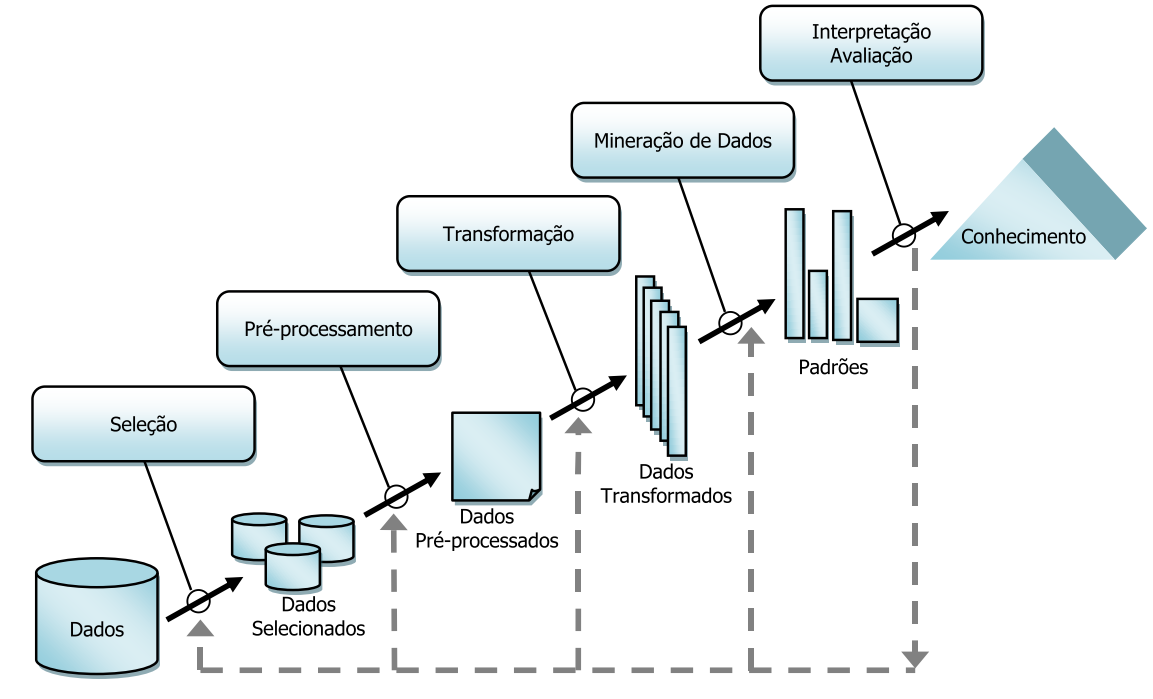
\includegraphics[scale=0.55]{Figuras/Etapas_KDD.png}
	\end{center}
    \legend{Fonte:\cite{Kampff2013}}
\end{figure}

\par
Por tanto ao termino da avaliação, o conhecimento extraído na mineração será introduzido e incorporado por outros sistemas, documentando e disponibilizando os métodos, afim  de apresentar o conhecimento obtido ao úsuario ou, mais importante de servir como suporte para a tomada de decisão \cite{Kampff2013}. Resumidamente, essas cinco etapas do processo de KDD podem ser classificadas em três categorias: pré-processamento, mineração de dados e pós processamento, como é apresentado na Figura 2 \cite{Fayyad1996}.

\begin{figure}[!htp]
	\begin{center}
    \caption{\label{fig:waveform_fig}As três partes da divisão do KDD segundo \cite{Fayyad1996}.}
	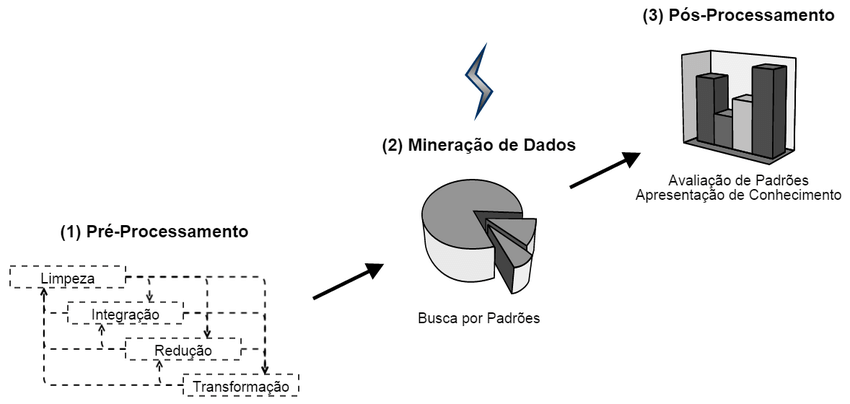
\includegraphics[scale=0.55]{Figuras/Tres_partes_KDD.png}
	\end{center}
    \legend{Fonte:\cite{Maciel}}
\end{figure}

\par
Como vimos antes, a aplicação de KDD, especificamente na etapa de mineração de dados, podemos perceber a sua enorme importância para todas as áreas que necessitem retirar informações de uma base forte e concreta de dados. Com isso, para a próxima seção, serão apresentados os conceitos relacionado a mineração de dados onde será aprofundado mais sobre essa fase explicando sua metodologia e tarefas de mineração.



%==========================
% MINERAÇÃO DE DADOS
%==========================

\section{Mineração de Dados}

O termo Mineração de dados(MD, do inglês, \textit{Data Mining}, DM), conhecido tambem como uma etapa de Descoberta de conhecimento em Bancos de Dados (KDD), pertence a disciplina que tem como objetivo de encontrar novas informações através da analise de grandes volumes de dados. No caso a frase \textbf{novas informações} esta se referindo ao processo de reconhecer novos conhecimentos, assim gerando mais descobertas científicas \cite{Baker2011}.

\par
Segundo \citeonline{Amaral2016}, a mineração de dados seria varios processos para explorar e anlisar grandes quantidades de dados na busca de padrões, previsões, erros, associações e entre outros. Em outras palavras, as ferramentas de MD examinam os dados, descobrem oportunidades escondidas ou problemas nos relacionamentos dos dados, e então identificam o comportamento dos negócios, envolvendo a mínima interferência do usuário, fazendo com que ele só se dedique a buscar o conhecimento \cite{Jefferson}. 

\par
Comumente a mineração de dados esta relacionada a aprendizagem de máquina, que na área de inteligência artificial desenvolve algoritmos capazes de fazer com o que o computador aprenda a partir do passado, isto é, ele aprende utilizando dados de eventos que já aconteceram \cite{Amaral2016}. Pode-se notar, que as ferramentas de mineração são baseados em algoritmos que formam contrução de blocos de inteligência artificial, redes neurais e entre outros, que ajuda a facilitar o trabalho de empresas os auxiliando a maximizar os seus lucros \cite{Jefferson}.

\par
Antes ninguém imaginaria que as aplicações de MD seria tão difundida em diversas áreas, pois, muitas delas não possuiam um modelo de dados armazenados digitalmente \cite{Amaral2016}. Hoje existe inúmeras técnicas e tarefas de mineração de dados que vem sendo utilizados com sucesso, em áreas como marketing por exemplo, para saber quais produtos um determinado cliente pretende comprar ou em medicina para prever qual paciente vai contrair um certa doença através do seu historico \cite{Martinhago2005}.

\par
Além de marketing e medicina, segundo \citeonline{Amaral2016} a mineração de dados e a aprendizagem de máquina são aplicadas em outras áreas como processamento de linguagem natural, bioinformática, reconhecimento de fala, detecção de fraude,  finanças, sistemas de recomendação, robóticas, mineração de textos, educação e entre outros. \textcolor{red}{No caso, neste trabalho, a mineração de dados educacional será abordado o seu conceito e importância na seção mais a adiante.}

\subsection{Tarefas de Mineração de Dados}

\par

As tarefas correspondem aos problemas que podem ser tratados pela mineração de dados. Depedendo do objetivo que se pretende alcançar a seleção da tarefa deve ser feita para se aplicar sobre a base de dados, existem inumeras tarefas, mas as que são mais utilizadas pela mineração podem ser classificadas como descrição (não-supervisionado) ou predição (supervisionado) \cite{Garcia2013, Camilo2009}.

\par
Segundo \citeonline{Santos2015}, na predição a análise é feita na forma de encontrar padrões repetidos e generalizados, com a finalidade de achar informações que estão escondidos nos dados. Já na descrição, existe argumentos já formulados onde se tenta procurar respostas que confirmem ou neguem esses argumentos, assim, verificando a sua veracidade. As tarefas mais comuns delas, são: 


\subsubsection{Associação}

\par
Uma tarefa de descrição, consiste em determinar quais items vão ser adquiridos diretamente em uma mesma transação, isto é, quanto um conjunto de atributos favorece para a presença de outro conjunto \cite{Garcia2013}. No caso se X existir alguma transação, há a possibilidade de Y existir também, pode ser apresentado na forma: SE \textit{atributo} X ENTÃO \textit{atributo} Y \cite{Camilo2009}. 

\par
Segundo \citeonline{Camilo2009}, a associação é uma das tarefas mais conhecidas pelo fato de terem tido ótimos resultados, principlamente na área de marketing com a análise de \textbf{Cesta de Vendas}, onde é identificados quais produtos são levados juntos pelo cliente. Pode-se perceber que são muito utilizado em estudos que tentam descobrir a relação entre os itens, para assim, criarem pacotes de venda ao consumidor \cite{Garcia2013}. 


\subsubsection{Classificação}

\par
Uma tarefa de predição, ela consiste em examinar uma certa característica nos dados (\textit{X}) e atribuir uma classe previamente definida (\textit{Y}), ou seja, visa identificar qual classe um determinado registro pertença, como podemos ver representada na Figura 3 \cite{Garcia2013, Kampff2013}. Exemplos disso é classificar se uma pessoa é de renda baixa, media ou alta, ou classificar se um cliente de um banco é bom ou mau pagador, assim determinando se deve conceder ou não creditos ao mesmo.

\begin{figure}[!htp]
	\begin{center}
    \caption{\label{fig:waveform_fig} Associação entre conjuntos de dados e classes.}
	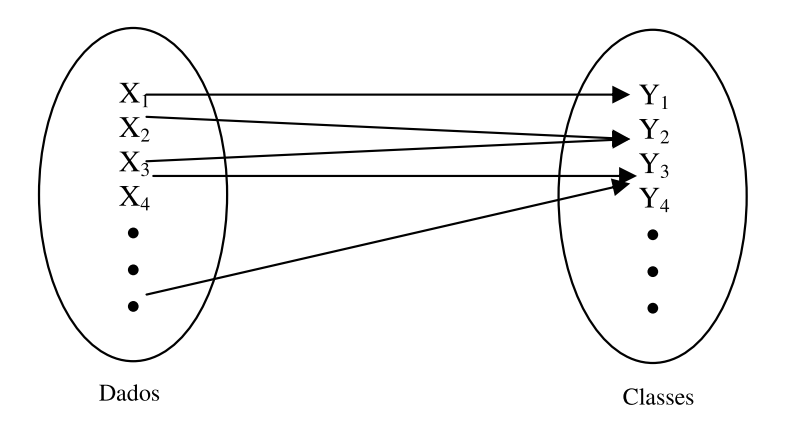
\includegraphics[scale=0.70]{Figuras/Classificacao.png}
	\end{center}
    \legend{Fonte:\cite{Rabelo2007}}
\end{figure}


\subsubsection{Regressão (Previsão ou Estimação)}

\par
Outra tarefa de predição, muito semelhante a anterior, só que com a diferença de que o atributo especial é identificado com um valor numérico e não categórico. Resume-se na estimativa do valor futuro de algum índice se baseando em dados do comportamento passado desse índice \cite{Camilo2009, LeandroSilva2014}. Exemplo, determinar se o índice da BOVESPA subirá ou descerá amanhã, prever o valor de vida de um equipamento, prever o desempenho do aluno, estimar a quantia a ser gasta por uma familia de quatro pessoas durante a volta às aulas e entre outros.

\par
A técnica de regressão pode ser classificada em linear e não-linear. Segundo \citeonline{Camilo2009}, são chamados de linear quando tanto as variáveis preditivas quanto as variáveis de resposta possui um comportamento linear em sua relação, por exemplo, quando um valor Y é uma função linear de X representado na Figura 4. Já a não-linear é o oposto da linear, é quando a relação entre as variaveis de resposta e predição não segue um comportamento linear, no caso, as relações entre as variaveis podem ser representada na forma de uma função polinomial. 

\begin{figure}[!htp]
	\begin{center}
    \caption{\label{fig:waveform_fig} Gráfico onde o valor y (pontuação alcançada) é uma função linear de x (horas de estudos).}
	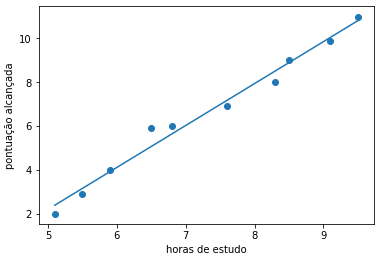
\includegraphics[scale=0.99]{Figuras/Regressao_linear.png}
	\end{center}
    \legend{Fonte:\cite{JoaoPaulo}}
\end{figure}

\subsubsection{Agrupamento (Clustering)}

\par
Outra tarefa de descrição, é um método de divisão de um conjunto de dados heterogêneos para um grupo homogêneo \cite{LeandroSilva2014}. Ele tende a reconhecer e aproximar os registros similares, isto é, ele junta um conjunto de registro semelhantes entre si que são diferentes de outros registros nos demais agrupamentos \cite{Camilo2009}. Clustering difere da classifição, pois, não necessita que os dados sejam previamente classificados (aprendizado não-supervisionado).

\par
Segundo \cite{Camilo2009}, o agrupamento não tem a intenção de predizer, estimar ou classificar uma varíavel, ele somente reconhece os grupos de dados iguais, como é demonstrado na Figura 5. Alguns exemplos de clustering como agrupar clientes por região do país ou com comportamento de compra similar, agrupar alunos com desempenho semelhantes, agrupar seções de usuários Web e entre outros.


\begin{figure}[!htp]
	\begin{center}
    \caption{\label{fig:waveform_fig} Registros agrupados em três clusters.}
	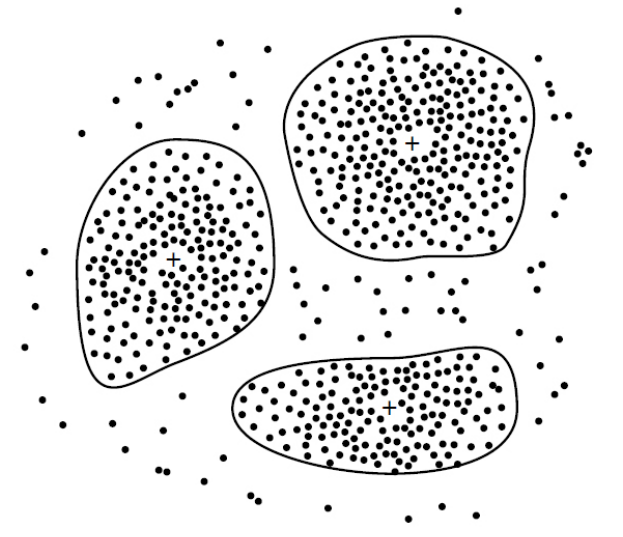
\includegraphics[scale=0.50]{Figuras/Agrupamento.png}
	\end{center}
    \legend{Fonte:\cite{Camilo2009}}
\end{figure}



\subsection{Mineração de Dados e Aprendizagem de Máquina}

\par
Como foi mencionado em tópicos anteriores, podemos perceber que a área de mineração de dados foi favorecido com diversos conceitos provenientes da área de aprendizagem de máquina, muito desses conceitos são visto em livros voltado para essa área, tais como as técnicas de classificação, regressão, associação e agrupamento. Os dois grupos principais de mineração de dados, predição e descrição, são parecidos com a forma em que os tipos de aprendizagens são divididos: Aprendizagem supervisionada e não-supervisionada.

\par
Por tanto na próxima seção tratara de alguns conceitos que já foram citados nesse capítulo, sendo que tais conceitos serão estudado de forma mais precisa, voltada para a área de aprendizagem de máquina.

%==========================
% APRENDIZAGEM DE MAQUINA - tecnicas(arvore de decisão, apriori...)
%==========================
\section{Aprendizagem de Máquina}

\par
Existem diversas atividades relacionadas ao conceito de aprendizagem, dificultando ainda mais a exata definição da palavra, tornando assim depedente de contexto. Porém, no contexto computacional, existe uma definição muito precisa de aprendizagem de máquina que pode ser dada \cite{Henke2011}. Segundo \citeonline{Alpaydin2009}, \textit{Machine Learning} são programas de computador que servem para melhorar um processo de um desempenho, utilizando dados de exemplo ou experiência passada.

\par
Em tese, se tem um modelo definido com alguns parâmetros, onde a aprendizagem é aplicada por um programa de computador para poder otimizar o parâmetro desse modelo utilizando dados de treinamento, sendo que, esse modelo pode ser preditivo, descritivo  ou os dois \cite{Alpaydin2009}. No caso, a aprendizagem de máquina utiliza o princípio da estatística na elaboração de seus modelos, porque, a tarefa principal está fazendo a dedução a partir de uma amostra. 

\par
Segundo \citeonline{Henke2011}, os algoritmos de aprendizagem podem ser a solução para resolver diversos problemas, pois, eles podem "aprender" a determinar padrões das classes que estão envolvidas no problema, através de exemplos existentes obtidos do ambiente. Conforme o modelo genérico da Figura 6 sobre aprendizagem de máquina ocorre o seguinte, o ambiente concede a informação para um elemento de aprendizagem, que utiliza essa informação para melhorar a base de conhecimento para que o elemento de desempenho a use na execução de sua tarefa. 

\begin{figure}[!htp]
	\begin{center}
    \caption{\label{fig:waveform_fig} Modelo genérico de aprendizagem de máquina.}
	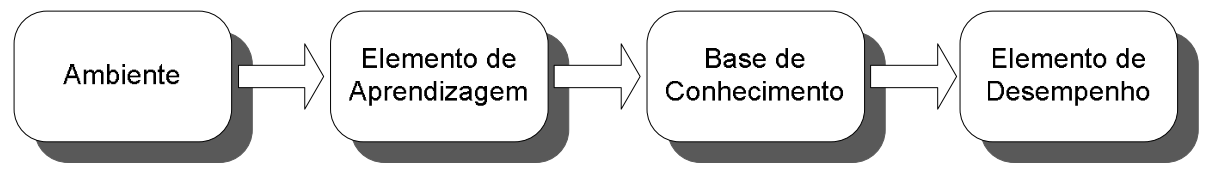
\includegraphics[scale=0.45]{Figuras/Modelo_Machine_Learning.png}
	\end{center}
    \legend{Fonte:\cite{Henke2011}}
\end{figure}

\par
Para a compreensão mais abrangente dos algoritmos de aprendizagem de maquina, é importante conhecer o conceito dos termos mais relevantes e mais usados segundo a nomenclatura abaixo de acordo com \cite{Monard2003, Souto2003, Henke2011}.

\begin{itemize}
    \item \textbf{Exemplo (padrão, instância):} É a ação ou o ato de se pegar um fato que já existe para explicar ou usar para alguma situação (por exemplo, para predição). Na maioria dos casos em aprendizagem de máquina, os exemplos são representados por vetores de características. Um exemplo uma amostra de tecido de um paciente.
    \item \textbf{Característica (atributo, variável):} É utilizado na descrição de um padrão (exemplo). Um atributo possui o seu tipo definido em um domínio, que indica os valores que ele pode apresentar (assumir). Exemplo, nível de expressão de um gene do tecido.
    \item \textbf{Vetor de características:} É quando um exemplo é descrito por uma lista de características. Um exemplo que se pode dar é um vetor m-dimencional que descreve para cada m genes, a medida do tecido de um certo paciente.
    \item \textbf{Classe:} Uma classe contém objetos parecidos, enquanto em outra classe possui objetos diferentes da dela. No caso de aprendizagem supervisionado, todo exemplo sempre possui pelo menos uma variável especial que descreve o fenômeno de interesse. Exemplo, as classe poderiam ser a preseça ou a ausência de câncer no tecido.
    \item \textbf{Conjunto de exemplos (conjunto de dados):} É formado por uma quantidade de exemplos (padrões) com seus determinados valores de atributos, onde, em aprendizagem de máquina, cada exemplo é relacionado a uma clase. Geralmente, ele é dividido em dois subconjuntos separados: o conjunto de treinamento e o conjunto de teste.
    \item \textbf{Acurácia (taxa de erro):} Seria a porcentagem de erros ou acertos efetuados pelo modelo para um determinado grupo de dados. No geral, a acurácia é aplicada em testes em que em nenhum momento não foram utilizados durante o processo de aprendizagem. Existem outros meios com técnicas mais complexas na estimação da acurácia como \textit{cross-validation} e \textit{bootstrap}. 
    \item \textbf{Falso positivo:} Suponhamos que temos duas classes, A seria positivo e B negativo, o falso positivo seria a quantidade de exemplos da classe B clasificados como da classe A. Já o falso negativo seria o oposto, a quantidade de exemplos A classificados como da classe B. Um exemplo bom onde ocorre isso é em matriz de confusão. 
    \item \textbf{Ruído:} Nenhum conjunto de dados é perfeito, é comum em que qualquer ambiente, acabar trabalhando com dados imperfeitos, no caso esses dados imperfeitos são conhecidos como ruído. Então, ele é definido como um conjunto de dados que aparentemente é inconcistentes comparado com o restante dos dados existentes. 
    \item \textbf{Overfitting (super-ajustamento):} É um termo que é utilizado para descrever quando um modelo se ajusta (especializa) muito bem ao conjunto de dados utilizados no seu treinamento, mas se torna ineficaz para prever novos resultados demonstrando uma taxa de acurácia baixa.
\end{itemize}

\subsection{Tipos de Aprendizagem}

\par
Segundo \citeonline{Henke2011} a aprendizagem de máquina pode ser dividido em dois tipos principais de aprendizagem: aprendizagem com professor e aprendizagem sem o professor.

\subsubsection{Aprendizagem com Professor}

\par
Conhecido tambem como aprendizado supervisionado, nele se tem a figura de um professor externo, no qual apresenta o conhecimento do ambiente através de um conjunto de exemplos de pares de entrada e saída, onde são propagados em uma sequência de regras que a máquina acompanhara para se obter o efeito desejado \cite{Lorena2007, Henke2011}.

\par
Exemplos desse tipo de aprendizagem, no caso de regressão, dado uma imagem de uma pessoa, através dos dados da imagem fornecido temos que prever a sua idade. Em classificação, dado um exemplo de tumor cancerígeno, temos que prever através da idade e do tamanho do tumor do paciente se ele é maligno ou benigno \cite{Pedro}.

\subsubsection{Aprendizagem sem Professor}

\par
Nesse não existe a presença de um professor, ou seja, não há exemplos rotulados de alguma fução para ser aprendida \cite{Lorena2007, Henke2011}. Nessa aprendizagem são identificados dois tipos de subdivisão:

\begin{itemize}
    \item \textbf{Aprendizagem por reforço:} Não se sabe qual a saída correta. Ele se preocupa de como um agente deve agir em um ambiente de forma que potencialize alguma noção de recompensa a longo tempo. Como os pares de entrada e saída não são fornecidos, ele tenta encontrar uma maneira de mapeá-los através de uma interação contínua com o ambiente, para poder reduzir um índice escalar de desempenho \cite{Henke2011, Alpaydin2009}. 
    \item \textbf{Aprendizagem não-supervisionada:} Não existe padrões de saída desejada. O algoritmo aprende a agrupar ou representar as entradas submetidas de acordo com uma medida de qualidade. Esse tipo de aprendizagem é usada principalmente quando se quer encontrar padrões ou tendências que ajudem na compreensão dos dados, nela inclui estimação de densidade, formação de agrupamentos e dentre outros \cite{Henke2011, Lorena2007}.
\end{itemize}

\par
Exemplo de aprendizagem não-supervisionada, no caso de agrupamento, dado um determinado conjunto de 1000 pesquisas de uma universidade, queremos encontrar um jeito de agrupar automaticamente elas de acordo com suas semelhaças ou relações por diferentes variáveis, tais como frases, sequêncis das palavras, contagens de páginas e etc \cite{Pedro}. Já na aprendijazem por reforço, temos como exemplo jogos, robôs e navegação.


\subsection{Algoritmos de Aprendizagem}

\par
Existe uma extensa quantidade de algoritmos disponíveis para classificação/regressão em aprendizagem de maquina, sendo que serão falados apenas alguns dos principais que são mais utilizados. Todos os algoritmos que serão mencionados abaixo, podem ser utilizados tanto para classificação quanto para regressão. \textcolor{red}{Avore de decisão - supervisionado, KNN - supervisionado, redes neurais - supervisionado, naive bayes - supervisionado, SVM - supervisionado.}


\subsubsection{Árvore de Decisão}

\par
Árvore de decisão (\textit{Decision Trees}) é uma ferramenta de aprendizagem que pode ser utilizada para tomada de decisão e dedução de valores categóricos. A ideia é de um aprendizado indutivo: se cria uma hipótese constituída em instâncias específicas que gera conclusões gerais \cite{Marques2014}. As árvores de decisão pegam como entrada um caso representado por um conjunto de atributos que retorna a uma decisão, que é a categoria para o valor de entrada


\par
Uma árvore é composta por três elementos importantes: os nós internos representam diferentes características, os ramos entre esses nós representam a possíveis valores que essas características podem possuir, enquanto os nós folhas representam o resultados, no caso, os valores de classificação da aplicação \cite{Henke2011, Barros2012}. Segundo \citeonline{Barros2012}, para a relização da classificação, deve ter uma tupla correspondente às características dos fluxos, que percorre pela árvore do nó raiz até  todos os nós folhas.  

\par
Para o melhor entendimento do processo de classificação de uma árvore de decisão, a Figura 7 mostra um exemplo usado no treinamento de dados para a tarefa de detecção de intrusão. De início, uma base de dados é fornecido ao algoritmo, onde, ele gera uma árvore feita para separar as amostras da classe Maligna de amostras da classe Benigna. Depois da construção da árvore, os dados novos podem ser fornecidos ao classificador, ao qual concedera uma das duas classes à amostra testada \cite{Henke2011}. 

\begin{figure}[!htp]
	\begin{center}
    \caption{\label{fig:waveform_fig} Treinamento dos dados em uma Árvore de Decisão.}
	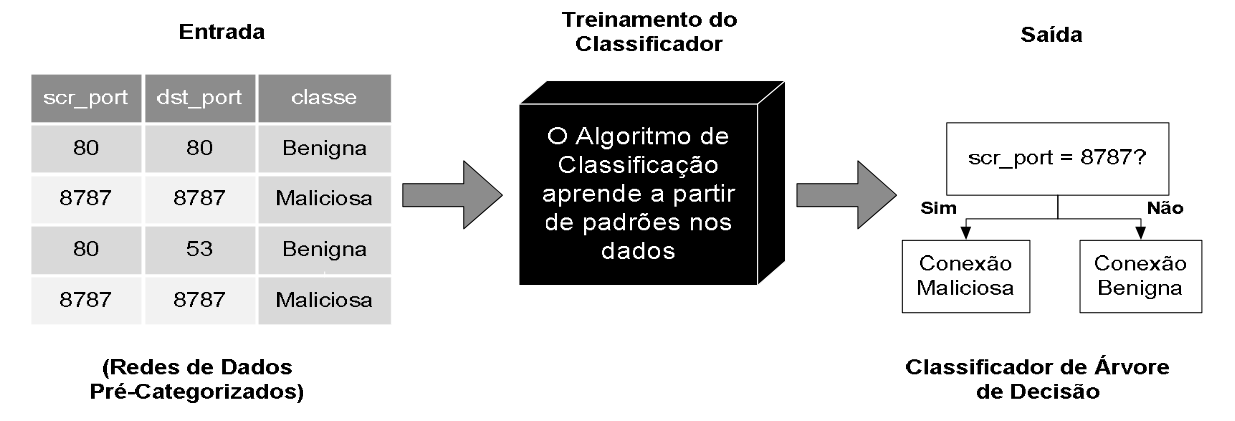
\includegraphics[scale=0.50]{Figuras/Arvore_decisao.png}
	\end{center}
    \legend{Fonte:\cite{Henke2011}}
\end{figure}

\par
Pelo que podemos perceber em um ponto de vista de decisão de negócios, uma árvore de decisão é uma quantidade mínima de perguntas sim ou não que alguem tem que perguntar, para poder avaliar a possibilidade de fazer uma decisão correta a maior parte do tempo. Como ferramente, possibilita tratar o problema de forma estruturada e sistemática para chegar a uma conclusão lógica \cite{Sara}. 


\subsubsection{K-\textit{Nerarest Neighbor} (KNN)}

\par
O algoritmo de KNN ou K-Vizinho Mais Próximo é um potente algoritmo não-paramétrico de classificação e regressão, utilizado desde 1950 na área da estatística \cite{Carvalho2014}. Segundo \citeonline{Henke2011}, ela é uma técnica baseada em instâncias, que constitui em atribuir a classe de cada elemento novo a partir da classe dominante conseguida através de seus vizinhos mais proximos, detectado no conjunto de treinamento. A definição de vizinhança é feita segundo a uma medida de distância estimado no espaço de atributos, exemplo de medida é a Euclidiana. 

\par
Por exemplo, queremos determinar a renda de uma pessoa de uma região, pesquisando k=20 vizinhos mais próximos desse indivíduo, podemos obter a renda através de valores dos atributos bairro, moradia, profissão, escolaridade e idade. Um de alguns problemas dessa técnica é a necessidade de se ter um número de atributos bastante razoavél para a determinação da vizinhança, e tambem, esse processo de classificação pode ser bastante cansativo para a máquina quando o conjunto de treinamento tem bastante dados \cite{Cortes2002, Henke2011}.

\subsubsection{Naive Bayes}

\par
Essa técnica de aprendizagem de máquina se baseia em fundamentações simples, mas que constantemente gera uma alta taxa de classificação em questões reais, como por exemplo, uma resposta para tal questionamento, como, qual a chance de um ataque ser de um determinado tipo, dado alguns acontecimentos do sistema observado? \cite{Henke2011}. Segundo \citeonline{Barros2012}, naive bayes analisa as categorias de aplicação para cada instância e relações dos atributos, derivando a probabilidade para cada relação delas entre seus valores.

\par
Segundo \cite{Henke2011}, uma de suas principais vantagens é a baixa complexidade na fase de treinamento, sendo que essa fase envolve somente os cálculos de frenquência para que as probabilidades sejam conseguidas. Em aplicações online, como problemas envolvendo segurança de redes, cujo, treinamento deve ocorrer online e com frequência continua, por ela ter essa característica naive bayes é muito indicada. Outra característica importante para segurança de redes, é o fato de ela poder manipular atributos nominais e numérico.

\par
O modelo de Naive Bayes é simples de construir e principalmente útil para grandes volumes de dados. Além de fácil, ele é conhecido também por ganhar de técnicas de classificação que são mais sofisticadas \cite{Sunil}. Naive Bayes utiliza o teorema de bayes que fornece uma forma de calcular a probabilidade posterior P(A|B) a partir de  P(A|B), P(A) e P(B). Observe a \autoref{eq:Bayes} abaixo:

\begin{equation}
    \label{eq:Bayes}
        {P(A|B)\quad =\frac { P(B|A)\quad *\quad P(A) }{ P(B) } }
\end{equation}

\par
Segundo \citeonline{Thiago}, precisamos dos seguintes dados utilizado na \autoref{eq:Bayes}, que são:
\begin{itemize}
    \item \textbf{P(A|B):} É a probabilidade posterior da classe (B, alvo) dada preditor (A, atributos), ou seja, a probabilidade de A acontecer dado que B ocorreu.
    \item \textbf{P(B|A):} É a probabilidade que representa a probabilidade de preditor dada a classe, ou seja, a probabilidade de B acontecer dado que A ocorreu.
    \item \textbf{P(A):} É a probabilidade original da classe, ou seja, a probabilidade de A ocorrer.
     \item \textbf{P(B):} É a probabilidade original do preditor, ou seja, a probabilidade de B ocorrer.
\end{itemize}

\subsubsection{Redes Neurais}

\par
Redes Neurais é uma técnica originado da psicologia e neurobiologia, que compõe basicamente de simulações baseada no comportamento dos neurônios \cite{Camilo2009}. Tal ideia vem da seguinte razão: o cérebro é tipo um aparelho que processa a informação com inúmeras habilidades, tais como por exemplo, o reconhecimento de voz, visão e etc. Por tanto, uma rede neural é bastante conectada por varias unidades (nó) como os neurônios, do qual a saída é uma combinação de varias entradas para outros neurônios \cite{Henke2011, Barros2012}.

\par
Segundo \cite{Carvalho2014}, na área de aprendizagem de máquina os algoritmos de redes neurais artificial são considerados poderosos, sendo que, são usados na resolução de problemas lineares e não-lineares, tendo apoio tanto no aprendizado supervisionado quanto no não supervisionado. Sua utilização mais constante é na solução de problemas não-lineares de classificação, através de uma estrutura conhecida com \textit{Multi-Layer Perceptron} (MPL) que sempre trabalha em conjunto nessa aréa de aprendizagem com o algoritmo mais conhecido, o algoritmo de Retropropagação (\textit{Backpropagation)}.

\par
Em bases de dados que possuam muitos ruído, que no caso são as inconsistências encontradas no conjunto de dados de treinamento, a técnica de redes neural é bastante recomendada. Pois, eles conseguem ser relativamente quase imunes a este ruídos, diferentes de outros modelos de aprendizagem supervisionado como árvore de decisão que são severamente afetados por esses ruídos \cite{Carvalho2014}. A Figura 8 logo depois, apresenta as diversas camadas que podem ser criadas em um processamento de uma rede neural \cite{Cortes2002}.

\begin{figure}[!htp]
	\begin{center}
    \caption{\label{fig:waveform_fig} Representação de um processamento de uma rede neural.}
	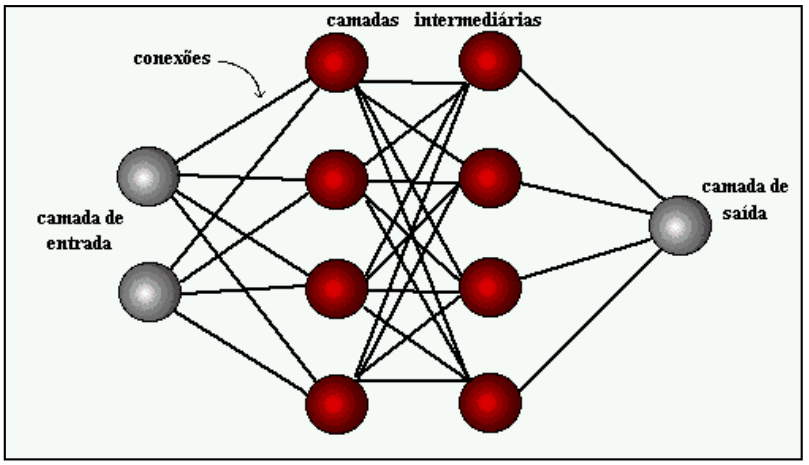
\includegraphics[scale=0.56]{Figuras/Redes_neural.png}
	\end{center}
    \legend{Fonte:\cite{Cortes2002}}
\end{figure}

\par
Segundo \citeonline{Cortes2002}, apresentado na Figura 8, todas as camadas intermediárias simbolizam os diferentes níveis de conhecimento que são obtidos no processo de seu percurso, numa tentativa de copiar o cérebro humano. Apesar de ser uma técnica poderosa, redes neurais é pouco utilizado em mineração de dados, pelo fato de seus algoritmos serem em sua maioria, incopreensíveis e também a função de aprendizado ser consideravelmente lenta, devido as várias interações que o algoritmo de retropropagação realiza para atualizar os valores da rede \cite{Carvalho2014}. 



\subsubsection{Support Vector Machines (SVM)}

\par
Máquina de vetores de suporte é um algoritmo supervisionado que é usado para o trabalho de classificação, onde ele utiliza um hiperplano como separador de classes. Este hiperplano é encontrado através da utilização do conjunto de treinamento (vetores de suporte) e ele trabalha como uma base para o limite da decisão ao classificar \cite{Costa2012}. Segundo \citeonline{Henke2011}, ela é uma técnica de classificação bastante aplicada em problemas de segurança, como por exemplo na detecção de \textit{phishing} e detecção de intrusos.

\par
O funcionamento do SVM pode ser dito da seguinte forma: se tem duas classes e um conjunto de treinamento onde as amostras pertencem as classe, a máquina vetor de suporte cria um hiperplano (conhecido como hiperplano de separação ótima) que divide o espaço de atributos em duas regiões, potencializando a margem de separação entre as mesmas. As amostras que antes não eram conhecidas são mapeadas para esse mesmo espaço e depois atribuídas a uma das classes \cite{Henke2011}.

\begin{figure}[!htp]
	\begin{center}
    \caption{\label{fig:waveform_fig} Dados de treinamentos representando alunos que passaram (círculos brancos) e não passaram (círculos cinzas) em uma disciplina.}
	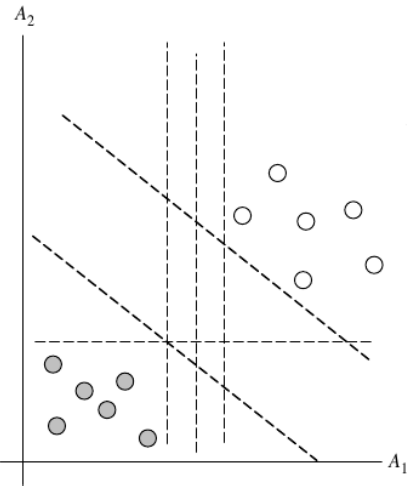
\includegraphics[scale=0.60]{Figuras/SVM.png}
	\end{center}
    \legend{Fonte:\cite{Costa2012}}
\end{figure}

\par
Como exemplo acima na Figura 9, suponhamos que os dados de treinamento sejam referentes aos alunos de uma turma com suas informações, apresentados como círculos, como a quantidade de postagens em um fórum de discussão (variável preditora). Além que, os dados representam cada aluno conforme o seu desempenho na disciplina (variável preditiva), alunos que passaram (círculos brancos) e que reprovaram (círculos cinzas). A priori, a meta do SVM é encontrar a melhor maneira de separar os dois grupos de alunos \cite{Costa2012}.



\par
Pode-se notar que existe uma quantidade infinita de hiperplanos que são representas na Figura 9 como essas linhas tracejadas, que podem separar as classes demonstradas que no caso são os círculos brancos e círculos cinzas. Então o propósito da máquina vetor de suporte é de encontrar o melhor hiperplano que maximize a distância entre elas das classes vizinhas. Um exemplo do melhor hiperplano para os dados que foram mostrado na Figura 9 encontrado pelo SVM é apresentado na Figura 10 \cite{Costa2012}. 


\begin{figure}[!htp]
	\begin{center}
    \caption{\label{fig:waveform_fig} Representação do melhor hiperplano que separa as classe, encontrado pelo algoritmo de SVM.}
	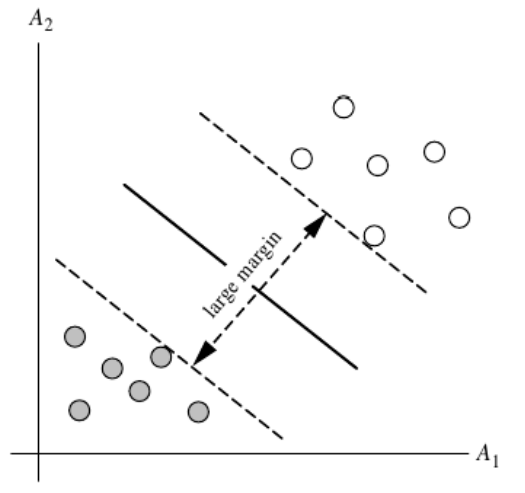
\includegraphics[scale=0.60]{Figuras/SVM_2.png}
	\end{center}
    \legend{Fonte:\cite{Costa2012}}
\end{figure}


\par
Embora SVM seja uma técnica recente, ela tem atraído muita atenção pelos seus resultados como: a possibilidade de modelar casos não-lineares difíceis gerando modelos de simples compreensão, consegue altos índices de assertividade, pode ser usada tanto para relações lineares quanto relações não lineares e entre outros \cite{Camilo2009}. Ultimamente um dos problemas dessa técnica é o tempo que se usa no aprendizado e muitas pesquisas estão se concentrando neste aspecto. 




%==========================
% MINERAÇÃO DE DADOS EDUCACIONAIS
%==========================

\section{Mineração de Dados Educacionais}

\par
Há pouco tempo, com o crescimento dos cursos a distância e também com aqueles que usam suporte computacional, muitos cientistas da área de Informática na Educação, têm demonstrado interesse em usar a mineração de dados para solucionar perguntas científica na área da educação \cite{Baker2011}. Nesse contexto, uma nova área de pesquisa surgiu denominada como Mineração de Dados Educacionais.

\par
A área de MDE (do inglês, \textit{Educational Data Mining}, EDM), é uma área que tem como proposito de desenvolver ou adaptar técnicas e algoritmos de mineração de dados existentes na literatura, de tal modo que sirvam a entender melhor os dados educacionais, gerados principalmente por professores e estudantes, tais como AVAs (Ambiente Virtual de Aprendizagem), STIs (Sistemas de Tutores Inteligentes), entre outros \cite{Costa2012, Marques2014}.

\par
Segundo \citeonline{Coutinho2016}, a MDE tem como apoio de disponibilizar a descoberta de conhecimentos que sejam importantes, único e útil, tais como: identificar padrões entre alunos, analisar o desempenho através de predição e a identificar perfis de forma que auxilie a gestão qualitativa da EAD. Os trabalhos nessa área, estão bastante concentrados em situações relacionados a um tipo específico de instituição, no caso, as Istituições de Ensino Superior (IES).

\par



% ----------------------------------------------------------
% Revisão de Literatura
% ----------------------------------------------------------
\chapter{TRABALHOS CORRELATOS}
\label{chapter:correlatos}

\par
\textcolor{red}{Neste capítulo serão apresentados alguns trabalhos relacionados que envolvem mineração de dados...} 

\section{Mineração de Dados Educacionais nos Resultados do ENEM de 2015}

\par
O trabalho de \citeonline{Simon2017} tem como objetivo em gerar um modelo preditivo da base de desempenho médio na área de ciências da natureza e suas tecnologias dos alunos de escolas do ensino médio, baseado nos dados públicos obtidos do Exame Nacional do Ensino Médio (ENEM) de 2015. Tal motivação foi pelo fato do cenário preocupante do baixo desempenho dos alunos do ensino básico no Brasil, conforme os dados de 2015 do PISA (\textit{Programme for International Students Assessment}).

\par
Segundo \citeonline{Simon2017} foi feito o pré-processamento dos dados do ENEM fornecidos pelo INEP, sendo que para cada área avaliada apresentavam-se 25 colunas que representavam uma informação ou variável, onde cada uma delas eram divididas em três categorias: características da escola, indicadores e desempenho. Das 25 variáveis, apenas 9 foram selecionadas como importante para a mineração de dados conforme o indicador da coluna Id representado na Figura 11. 

\begin{figure}[!htp]
	\begin{center}
    \caption{\label{fig:waveform_fig} Variáveis disponibilizadas pelo ENEM por escola.}
	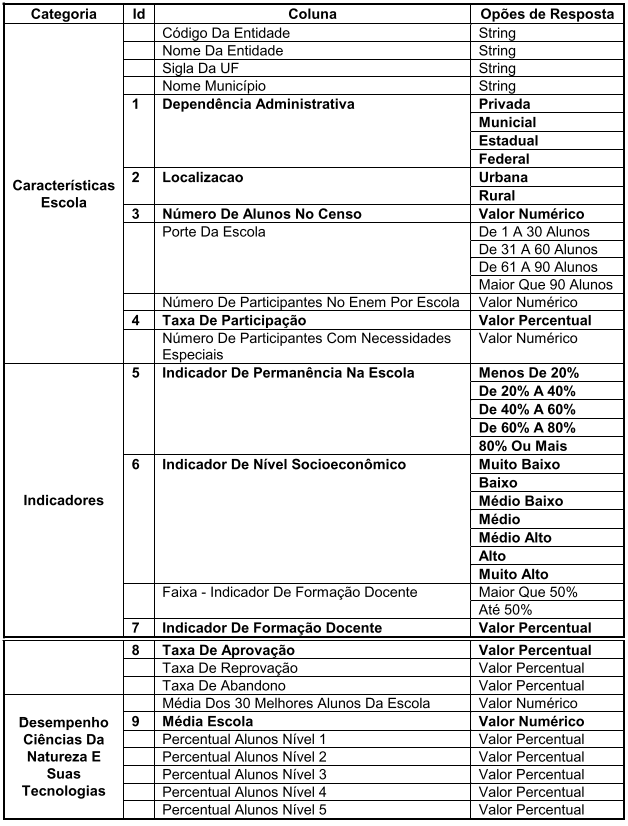
\includegraphics[scale=0.99]{Figuras/Tabela_ENEM.png}
	\end{center}
    \legend{Fonte:\cite{Simon2017}}
\end{figure}

\par
\citeonline{Simon2017} destacaram que a variável Média Escola indicava o desempenho médio dos alunos da escola na área de ciências da natureza e suas tecnologias, onde esses dados eram fornecidos como valor numérico pelo INEP, então para facilitar a mineração dos dados, ele teve que converte-lo para uma categoria mais limitada que foi dividida em quatro valores possíveis, segundo a escala prevista pelo INEP conforme a Figura 12. Os dados fornecido pelo INEP, vinham em uma planilha no formato .xlsx e teve que ser convertido para .csv, pois, o formato não era suportado pelo software WEKA.


\begin{figure}[!htp]
	\begin{center}
    \caption{\label{fig:waveform_fig} Categoria para os valores Média Escola.}
	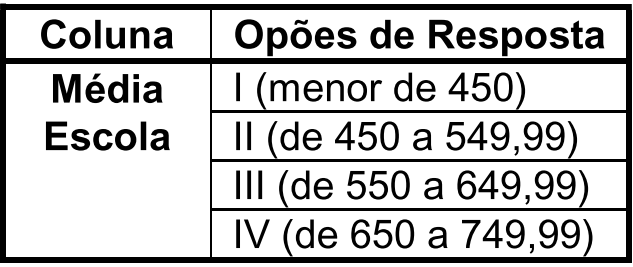
\includegraphics[scale=0.50]{Figuras/Tabela_ENEM_2.png}
	\end{center}
    \legend{Fonte:\cite{Simon2017}}
\end{figure}

\par
Relacionando os fatores socioeconômicos e o índice de desempenho médio em ciências da natureza e sua tecnologias dos alunos, \citeonline{Simon2017} construiu um modelo preditivo utilizando a técnica de mineração de árvore de decisão. Tal técnica, usou o algoritmo j48 através do software WEKA, que foi executado utilizando a opção de \textit{cross-validation}, onde o valor para \textit{fold} era igual a 10 e com a variável depedente Média Escola. Com a árvore obtida, demonstrou como variável independente mais relevante foi a variável Tipo Escola, que se divide entre quatro valores: privada, federal, estadual e municipal.

%Variavel dependete seria o resultado e a variavel independente seria o caminho que ele iria percorre até o resultado. Exemplo: variavel dependete (aluno passou | aluno não passou), variavél independente(entregou os trabalhos, participou das aulas, tirou nota boa na prova, numeros de faltas e etc).

\par
Depois da variável Tipo Escola, a variável hierarquicamente seguinte é a Nível socioeconômico e a partir dela as váriaveis seguintes se alternam de posição conforme as funções dos valores dos níveis superiores. Como resultado, sobre o desempenho médio dos alunos na área de ciências da natureza e suas tecnologias, as categorias que mais se destacaram foram a III e IV, acima de 550 pontos, que ocorreram nas escolas: privadas e estaduais com o nível socioeconômico muito alto, federais com o nível médio alto e muito alto e municipal com o nível médio alto.

\par
\textcolor{red}{Há alguns pontos deste trabalho que se relacionam ao trabalho que pretendo fazer, uma delas é a base de dados dos fatores socioeconômico e outras informações fornecidos do ENEM pelo INEP, que esta relacionado na parte de pré-processamento, é semelhante aos dados fonecidos pela Comissão Permanente do Vestibular (CPV) da UFRR, como base eu poderia pegar as mesmas variáveis que foram escolhidas no trabalho de \citeonline{Simon2017} para agilizar o meu trabalho de minerar os dados mais imporntante para solucionar o meu problema.}
\par
\textcolor{red}{Outro ponto importante é o modelo preditivo que ele abordou, que é a técnica de mineração de árvore de decisão que utiliza o algoritmo J48 do software WEKA, já que eu utilizarei a mesmo conceito de modelo, poderia utilizar a opção de \textit{cross-validation}, no caso o K-\textit{folds}, que ele usou para os treinos e testes dos dados para a validação do modelo.}



\section{Prática de Mineração de Dados no Exame Nacional do Ensino Médio}

\par
O trabalho de \citeonline{Silva2014}, apresenta um estudo de mineração de dados educacionais, mais especificamente, utilizando a tarefa de Associação de Dados de MD no intuito de encontrar padrões de regras nos dados dos questionários socioeconômicos e resultados das provas do Exame Nacional de Ensino Médio (ENEM), fornecidos pelo INEP. O objetivo é de executar as etapas do KDD para o processamento dos dados do ENEM, de modo que por consequência, se utilize a técnica de associação para se encontrar regras proporsicionais que relacionam os fatores socioeconômicos do candidato com o seu desempenho na prova.

\par
Para o trabalho de \citeonline{Silva2014}, foi utilizado o banco de dados com os questionários socioeconômico e os desempenhos da prova do ENEM de 2010, fornecido pelo INEP, onde, para acessar os dados do banco dele, foi usado os softwares Oracle Express Edition 11g e PL/SQL Developer que permitem a extração dos dados que foram determinado para o foco da pesquisa. Os dados utilizados para fazer a mineração de dados, foi da região Sudeste das suas capitaias: Vitória, Belo Horizonte, São Paulo e Rio de Janeiro.

\par
Na parte de pré-processamento, foi selecionado somente os dados das capitais do Sudeste que resultaram em 452.710 alunos, que entretanto, foram eliminados 310.000 alunos das quatros capitais, pois, eles não compareceram no dia da prova. As questões selecionadas para a pesquisa  foram de quantas pessoas moravam com o candidato, a renda familiar mensal, o nível de escolaridade da mãe e o tipo de escola que cursou no ensino médio. Sendo que essas questões foram analisadas para saber se contribuia, interferia ou afetava a nota e o desempenho do candidato na prova.

\par







%==========================================================
% REVISÃO SISTEMÁTICA
%==========================================================
\section{Revisão sistemática}
A revisão sistemática consiste em um método de identificação, analise e interpretação de pesquisas relevantes em determinada área ou questão de pesquisa. Para execução da revisão sistemática requer esforço maior, em comparação as pesquisas tradicionais, sendo necessário seguir uma sequência de passos metodológicos sobre a área ou questão de pesquisa ao qual deseja ser feita a pesquisa\cite{kitchenham2004procedures}.

Para a execução da revisão sistemática, é necessário um esforço considerável, se comparado a uma revisão informal a literatura. Enquanto que a revisão de literatura informal é conduzida de forma ad-hoc, sem planejamento e critérios de seleção estabelecidos a priori, a revisão sistemática requer um protocolo formal bem definido, com uma sequência de passos metodológicos, para conduzir uma pesquisa sobre o tema ao qual deseja-se realizar a pesquisa \cite{MafraTravassos}.

A aplicação da revisão sistemática requer que seja seguido um conjunto bem definido e sequencial de passos, seguindo um protocolo de pesquisa desenvolvido previamente. Através deste método é possível realizar uma extensa pesquisa, contemplando uma grande quantidade de informações sobre o assunto pesquisado\cite{MafraTravassos}. Este protocolo é construído considerando um tema específico que representa o elemento central da investigação, onde os passos da pesquisa, as estratégias definidas para coletar as evidências e o foco das questões de pesquisa são definidas explicitamente, de tal forma que outros pesquisadores sejam capazes de reproduzir o mesmo protocolo de pesquisa\cite{biolchini2005systematic}.

Segundo \cite{MafraTravassos}, o processo para a condução de revisões sistemáticas envolve três etapas:
\begin{enumerate}
\item \textbf{Planejamento da Revisão:} os objetivos da pesquisa são listados e o protocolo da revisão é definido.
\item \textbf{Condução da Revisão:}nesta atividade, as fontes para a revisão sistemática são selecionadas, os estudos primários são identificados, selecionados e avaliados de acordo com os critérios de inclusão, exclusão, e de qualidade estabelecidos durante o protocolo da revisão.
\item \textbf{Análise dos Resultados:} os dados dos estudos são extraídos e sintetizados para análise e apresentação
dos resultados.
\end{enumerate}

Entretanto, como o objetivo deste trabalho é realizar um estudo exploratório de caracterização de área podemos dizer que esta revisão sistemática se caracteriza como uma quasi-sistemática \cite{travassos2008environment}, pois segue o mesmo processo da revisão sistemática e preserva o rigor e mesmo formalismo para as fases metodológicas de elaboração de protocolo e execução da revisão, mas sem a aplicação de uma meta-análise a princípio, que pode ser aplicada posteriormente.

%==========================================================
%PLANEJAMENTO DA REVISÃO SISTEMÁTICA
%==========================================================
\subsection{Planejamento da Revisão Sistemática}
\textbf{Objetivo:} Este estudo tem o objetivo esquematizado a partir da estrutura do paradigma GQM (do ingles \textit{Goal,Question and Metric})\cite{basili1994experience}.

\begin{table}[h!]
\centering
\label{}
\begin{tabularx}{\textwidth}{|l|X|}
\hline
Analisar & Publicações científicas através de um estudo baseado em revisão sistemática \\ \hline
Com propósito de & Identifica-las \\ \hline
Com relação as & Vantagens e desvantagens da utilização de assertiva e transformações de código na verificação do código na linguagem de descrição VHDL \\ \hline
Do ponto de vista do & Pesquisador \\ \hline
No contexto & Acadêmico ou industrial para verificação de assertivas na linguagem de descrição VHDL \\ \hline
\end{tabularx}
\caption{Objetivo do estudo utilizando o paradigma GQM}
\end{table}

\textbf{Formulação da Pergunta:} Buscamos respostas para as seguintes perguntas:
\begin{itemize}
\item \textbf{Q1:} Quais são os métodos para verificação de circuitos lógicos descritos na linguagem de programação VHDL?
	\begin{itemize}
	\item \textbf{Q1.1:} Foi desenvolvido e está disponível alguma ferramenta para aplicação do método?
	\item \textbf{Q1.2:} Qual a técnica de exploração de estados para circuitos lógicos?
	\item \textbf{Q1.3:} O método proposto é baseado em técnicas de verificação de software?
	\item \textbf{Q1.4:} Como o método proposto valida pré e pós condições no programa?
	\item \textbf{Q1.3:} Foi utilizado algum \textit{benchmark} de programas em VHDL para experimentação e o mesmo encontra-se disponível?
	\item \textbf{Q1.4:} Quais as perspectivas futuras para melhorar da aplicação do método proposto?
	\end{itemize}
\end{itemize}

\textbf{Escopo da pesquisa:}Na delimitação do escopo da pesquisa foram estabelecidos critérios, buscando garantir a viabilidade da execução, acessibilidade dos dados e abrangência do estudo realizado. A pesquisa dar-se-á a partir de bibliotecas digitais através das suas respectivas máquinas de busca e, quando os dados não estiverem disponíveis eletronicamente, através de consultas manuais.

\textbf{Critérios de Seleção de Fontes.}Para as bibliotecas digitais é desejado:
\begin{itemize}
\item Possuir uma máquina de busca que permita o uso de expressões lógicas ou mecanismo equivalente.
\item Incluir em sua base, publicações de exatas ou correlatas que possuam relação direta com o tema a ser pesquisado
\item As máquinas de busca deverão permitir a busca no texto completo das publicações.
\end{itemize}

Segundo \cite{rocha2015verificaccao}, os mecanismos de busca utilizados devem garantir resultados únicos através da busca de um mesmo conjunto de palavras-chaves (string de busca). Quando isto não for possível, deve-se estudar e documentar uma forma de minimizar os potenciais efeitos colaterais desta limitação.

\textbf{Métodos de Busca das Publicações.} As fontes digitais foram acessadas via Web, através de expressões de busca pré-estabelecidas. A biblioteca digital consultada foi a Scopus, acessível em http://www.scopus.com. Segundo a editora \cite{Elsevier}, a Scopus é uma das maiores bases de dados de resumos e citações da literatura de pesquisa \textit{peer-reviewed} com mais de $22,800$ títulos de mais de 5,000 editoras internacionais abrangendo as áreas de tecnologia, medicina, artes, ciências sócias e com atualizações diárias. Entre as editoras podemos citar: Springer \cite{Springer}; IEEE Xplore Digital Library \cite{IEEE};ACM Digital Library \cite{ACM} ; ScienceDirect/Elsevier \cite{B.V}; Wiley Online Library \cite{Sons}; dentre outras.

\textbf{String de Busca.} A string de busca foi definida segundo o padrão PICO (do inglês \textit{Population, Intervention, Comparison, Outcomes}) \cite{kitchenham2009systematic}, conforme a estrutura abaixo:
\begin{itemize}
	\item População: Trabalhos publicados em conferências e periódicos que relacionam verificação de propriedades de circuitos lógicos em códigos para a descrição de hardware.

	\item Intervenção: Verificação de propriedades relacionadas a verificação de circuitos para as diferentes estruturas das linguagens de descrição de hardware;

	\item Comparação: análise de cobertura e suporte das abordagens identificadas para a verificação de propriedades das linguagens de descrição de hardware;

	\item Resultados: a partir da descrição das abordagens pretende-se verificar a cobertura que cada abordagem apresenta na manipulação das diferentes estruturas da linguagem de descrição de hardware para a verificação de propriedades baseada em assertivas.
\end{itemize}

Segundo, \cite{rocha2015verificaccao}, como este estudo representa um estudo de mapeamento/caracterização, a string de busca foi definida de acordo com dois aspectos: População e Intervenção, como é apresentado na estrutura abaixo. Posteriormente esta mesma string de busca será executada na biblioteca Scopus para busca de artigos e publicações de modo a gerar uma interseção entre população e intervenção.
\begin{itemize}
\item População: publicações que fazem referência a verificação de propriedades de circuitos lógicos e sinônimos:
	\begin{itemize}
	\item \textbf{Palavras-chaves:} "circuit checker" OR "circuit verification" OR "contract based verification" OR "code analysis" OR "static analysis" OR "dynamic analysis" OR "safety verification" OR "RTL analysis" OR "program analysis" OR "property verification" OR "formal verification" OR "model checking" OR "model checker" OR "hardware checker" OR "hardware verification" OR "validity checker" OR "hardware assertion" OR "assertion checker" OR "assert verification" OR "assertion-based verification" OR "assertion based verification" OR "assertion-based design" OR "bit level verification"
	\end{itemize}
\item Intervenção: Verificação de circuitos e sinônimos:
	\begin{itemize}
	\item \textbf{Palavras-chaves:}"hardware statement" OR "hardware code" OR "hardware source code" OR "hardware semantics" OR "hardware property" OR "logical gates" OR "sequential circuit" OR "parallel circuit" OR "real circuits" OR "complex circuits" OR "control circuitry" OR ”software netlist” OR “hardware emulation” OR “silicon debug”
	\end{itemize}
\end{itemize}
%==========================================================
%PROCEDIMENTOS DE SELEÇÃO E CRITERIOS
%==========================================================
\subsubsection{Procedimentos de Seleção e Critérios}

A estratégia de busca será aplicada por um pesquisador para identificar as publicações em potencial. A seleção das publicações dar-se-á em 4 etapas, porém o terceiro filtro não foi executado nesta etapa do projeto, resumindo-se em apenas 3 etapas:
\begin{enumerate}
\item \textbf{Seleção e catalogação preliminar dos dados coletados:}A seleção preliminar das publicações será feita a partir da aplicação da string de busca na biblioteca Scopus, o resultado desta busca corresponde a seleção preliminar. Todas as publicações serão armazenadas para análise posterior;

\item \textbf{Seleção dos dados relevantes - [1 filtro]:} A seleção preliminar com o uso da expressão de busca não garante que todo o material coletado seja útil no contexto da pesquisa, pois a aplicação das expressões de busca é restrita ao aspecto sintático. Por isso, é necessário a criação de filtros de exclusão e inclusão, de modo a classificar os artigos e publicações que se enquadram no contexto da pesquisa realizada. Nesta epata apenas serão lidos o título, abstracts, e palavras-chaves e classificar de acordo com os filtros, ou seja, se será aceito ou excluído. Devem ser excluídas as publicações contidas no conjunto preliminar que:
	\begin{itemize}
	\item \textbf{CE1-01:} Não serão selecionadas publicações em que as palavras-chave da busca não apareçam no título, resumo e/ou texto da publicação (excluem-se os seguintes campos: as seções de agradecimentos, biografia dos autores, referências bibliográficas e anexas).
	\item \textbf{CE1-02:} Não serão selecionadas publicações em que descrevam e/ou apresentam ‘keynote speeches’, tutoriais, cursos e similares.
	\item \textbf{CE1-03:} Não serão selecionadas publicações em que o contexto das palavras-chave utilizadas no artigo leve a crer que a publicação não cita uma abordagem para verificação/validação de códigos para descrição de hardware.   
	\item \textbf{CE1-04:} Não serão selecionadas publicações em que o contexto das palavras-chave utilizadas no artigo leve a crer que a publicação não cita uma abordagem para verificação de código de descrição de hardware baseado em assertivas ou propriedades de verificação de hardware.
\end{itemize}

Podem ser incluídas apenas as publicações contidas no conjunto preliminar que:

	\begin{itemize}
	\item \textbf{CI1-01:}Podem ser selecionadas publicações em que o contexto das palavras-chave utilizadas no artigo leve a crer que a publicação cita uma abordagem para verificação de código de descrição de hardware baseado em assertivas ou propriedades de verificação de hardware.
	\item \textbf{CI1-02:}Podem ser selecionadas publicações em que o contexto das palavras-chave utilizadas no artigo leve a crer que a publicação cita recomendações de melhoria na utilização de abordagens para verificação de código de descrição de hardware baseado em assertivas ou propriedades de verificação de hardware.
	\end{itemize}
%=======================
%Filtro 2
%=======================
\item \textbf{Seleção dos dados relevantes - [2 filtro]:} Apesar do 1 filtro limitar o universo de busca, infelizmente não há garantias de que todo material selecionado no filtro anterior seja útil no contexto da pesquisa. Neste caso, novos filtros são gerados, buscando, da mesma forma que o primeiro filtro, classificar os artigos e publicações que se enquadram no contexto da pesquisa. Para este filtro é necessário a leitura na integras dos artigos selecionados anteriormente. O objetivo é identificar que relacionam assertivas e/ou propriedade de verificação de hardware.
    \begin{itemize}
    \item \textbf{CS2 -ASS -VER\_HARD:} Não devem ser selecionadas publicações que não contextualizem verificação de hardware e não citam assertivas
    \item \textbf{CS2 +ASS -VER\_HARD:} Não devem ser selecionadas publicações que não contextualizem verificação de hardware, mas citam assertivas
    \item \textbf{CS2 -ASS +VER\_HARD:} Não devem ser selecionadas publicações que contextualizam verificação de hardware, mas citam assertivas.
    \end{itemize}
Dessa forma, todas as publicações devem respeitar o critério abaixo:
	\begin{itemize}
	\item \textbf{CS3 +ASS +VER\_HARD:} Serão selecionadas publicações que contextualizam verificação de hardware e citam assertivas em seu contexto.
	\end{itemize}     	
\end{enumerate}

\par
\textcolor{red}{Devido ao tempo necessário para o desenvolvimento execução dos filtros da revisão sistemática serem extensos, apenas o primeiro filtro foi executado neste projeto, mesmo que os parâmetros para o segundo filtro já tenho sido desenvolvidos. Em contra partida foram selecionados 6 artigos que serviram como ferramentas de estudo para o desenvolvimento da metodologia que será apesentada no \autoref{chapter:metodo}.}

%====================================
%REVISÃO DA LITERATURA
%====================================
\section{Revisão da literatura}
Nesta sessão serão apresentados trabalho relevantes para o desenvolvimento do método proposto. Os artigos apresntam técnicas de transformações de código, utilização de \textit{Assertion-based verification} e PSL para verificação de hardware.

\subsection{V2c-A verilog to C translator}
O artigo apresenta um ferramenta implementada em C++ chamada \textit{v2c} para conversão de código da linguagem de descrição Verilog para linguagem de programação C. A ferramenta é executada a nivél de palavra, visto que esta abordagem garante uma aumento na escalabilidade, mas também proporionando que tecnicas, como interpolação e aceleração de loop possam ser utilizadas para verificação, algo inviavél, caso a tradução fosse executada a nível de bit. O sistema recebe como entrada um código em Verilg, onde são aplicadas regras semânticas e mapeando os bit de operação, chamado software netlist. Após isso, o código intermediário é convertido para C\cite{mukherjee2016v2c}.

\par
\textcolor{red}{A contribuição deste trabalho consiste na utilização de transformações de código como base principal e partindo deste pressuposto torna-se vantajoso devido a utilização de outras ferramentas que não apresente suporte a certas linguagens, tais com a ferramenta ESBMC, utilizada neste trabalho, não apresenta suporte a VHDL, porém apresenta suporte as linguagens C/C++. Em outras palavras ,a contribuição deste trabalho foi a utilização de traduções de códigos e utilizado este conceito como modelo de entrada para analise de circuitos.}

\subsection{Unbounded safety verification for hardware using software analyzers}
No artigo foi apresntado um metodologia essencial para o desenvolvimento deste projeto. O artigo aborda a utilização de técnicas de software e analisadores de software, com o objetivo de utiliação analises de hardware e software para analise de circuitos e com isso trançar um paralelo entre as abordagens. Para testes foram utilizadas três metodologias de analise, usando interpolação, \textit{k-induction} e tecnologias hibrídas. Como resultante dos destes, foi observado as principais causas de erros, por exemplo, bits não preciso e no caso das operações a \textit{bit-level} ocorria perda de informações. Também foi obeservado que apesar de não serem otimizadas para analises de hardware, alguns analisadores de softaware podem, dependendo da técnica utilizada no analisador,  ser tutilizada para analise de hardware\cite{mukherjee2016unbounded}.

\par
\textcolor{red}{No artigo foi apresentado um metodologia essencial para o desenvolvimento deste projeto, visto que a utilização de técnicas de analise de software para o desenvolvimento de analise de \textit{hardware} é o foco a ser abordado neste projeto de maneira prática. Entretanto, o objetivo deste projeto é a utilização de técnicas de software para analise de circuitos, diferente do artigo apresentado acima que busca utilização uma abordagem mais complexa provando a possibilidade da utilização de técnicas de analise de software no contexto da verificação de hardware.}

\subsection{Formal verification of timed VHDL programs}
O artigo apresenta analise de tempo relacionado a cada porta lógica dentro o circuito. A métodologia apresenta a traduçao de um circuito lógico codificado em VHDL para um formalismo baseado em automato de tempo. Tal formalismo é representado por uma automato de estados finitos com relogios simbólicos que evoluem em taxa uniforme.A tradução é executada de modo automatico, baseado na emulação da propagação de cada transação ao longo de cada sinal, o seuja, são automatos programados e cronometrados do circuito. Após a tradução para automato, a analise é feita pela ferramenta UPPAL, \textit{Model checking} de verificação de propriedades de tempo. Seguindo esta metodologia a analise pode ser extraida de modo independente de cada bloco, desta forma a anlise é feita de forma mais precisa, podendo ser analisado inumeros fatores, tais como limites de intervalo e sinal de correlação \cite{bara2010formal}.

\par
\textcolor{red}{O artigo apresenta uma abordagem de tempo, que torna-se interessante adição ao método. Porém até o momento a função não foi implementada ficando a trabalho futuros.}

\subsection{On the use of assertions for embedded-software dynamic verification}
O artigo apresenta metodologia para de integração dinamica de  \textit{Assertion-based verification} para varias fases de analise da verificação de fluxo em sistemas embarcados, por exemplo, emulação, diagnosticos e \textit{Debug}, mas também um ferramenta chamada \textit{RadCheck}. O metodo de aplicação, chamado \textit{V-model} é dividido em fases de verificação em paralelo com as fases de design do circuito. Com base no \textit{v-Model}, o metodo é aplicado, iniciando com o nível de sistema e as especificação do sistema, neste caso especificado usando PSL. Neste nível é especificado todas as funcionalidaes gerais da aplicação. No nivel de integração visa investigar problemas de interação que possam ocorrer, definindo propriedades que cobrem incrementalmente as unidades estruturais interativas de aplicação. No nível de unidade descrevem comportamentos internos e são definidas através de parâmetros de entrada / saída de unidade e estruturas de dados internas.\cite{di2012use}

\par
\textcolor{red}{A contribuição deste projeto esta relacionado a utilização de assertivas no contexto da verificação de software. As assertivas são o principal meio de analise proposto neste projeto, visto que estas mesma assertivas serão analisadas pelo ESBMC. Aliado a isso o artigo apresenta modelos de utilização de assertivas no processo de verificação de hardware, e tais assertivas foram adaptadas para um modelo próprio a ser utilizados no contexto deste projeto.}

\subsection{Incorporating efficient assertion checkers into hardware emulation}
\todo[inline]{Este foi o artigo que menos entendi, então tive uma pequena dificuldade para a escrita deste capitulo.}
\textcolor{red}{O artigo apresenta uma ferramenta de geração de assertivas no contexto da emulação de circuitos, de modo que estas assertivas descrita em PSL possam transformadas para o modelo de linguagem de descrição de hardware. Inicialmente é realizada toda analise de cada assertiva e a mesma é traduzida em partes, levando em consideração os operadores e cada estrutura, por exemplo if-else, utilizado na declaração da assertiva.\cite{boule2005incorporating}.}

\par
\textcolor{red}{O artigo apresenta aspectos importantes, tais como a utilização de uma ferramenta para geração de assertivas, o que torna-se no contexto deste projeto, extremamente importante, visto que o modelo adotado atualmente consiste tanto na geração automática das assertivas, bem como a inserção manual por parte do usuário.}


% ----------------------------------------------------------
% Detalhes de Desenvolvimento do Projeto
% ----------------------------------------------------------
\chapter{MÉTODO PROPOSTO}
\label{chapter:metodo}

\par
\textcolor{red}{Com a grande quantidade de dados que são armazenados dos seus acadêmicos, as faculdades muitas vezes não sabe em como utilizá-los para benefício próprio. Com base nesses dados armazendos, especificamente os dados do candidatos que prestaram o vestibular, se pretende aplicar a mineração de dados educacional, com o objetivo de extrair o conhecimento dessa base para saber quais fatores que afetam o desempenho desse candidato em sua nota do vestibular. Neste contexto o trabalho proposto segue as seguintes etapas para se alcançar esse objetivo.}

\par
\textcolor{red}{Para a fase de pré-processamento será analisado o banco de dados do vestibular da Universidade Federal de Roraima (UFRR) do ano de 2017 fornecido pela Comissão Permanente de Vestibular (CPV), que esta encarregada de gerenciar os dados geral dos candidatos inscritos. Para formar a base de dados onde será aplicado a mineração, estará sendo feita a junção dos dados dos questionarios socioeconômico que contém no total de 37 questões e os dados de cadastro geral que são realizados pelos candidatos durante a etapa de inscrição.}


\par
\textcolor{red}{Como em todo banco de dados é normal encontrar inconsistência de dados, como ruídos, itens de dados em branco, valores absurdos e erros de digitação, para grantir a qualidade dos dados, serão necessário corrigir esses problemas para que na hora da mineração não ocorra nenhum erro ou que tenha algum resultado incoerente. Tambem será necessario ser feito a eliminação de atributos repetidos assim como dados inrrelevantes para a pesquisa e dos dados de candidatos que não compareceram para prestar o vestibular.}

\par
\textcolor{red}{Depois de selecionar e transformar a base de dados em um formato apropriado, será aplicado a técnica de mineração de ávore de decisão para a análise de dados dos candidatos, a escolha desse método foi pelo seguinte motivo, que segundo \citeonline{Simon2017}, esta técnica serve como um sistema de suporte a decisão, que é utilizado para aprender funções de classificação que mostra o valor de uma variável dependente por meio de dados de variáveis independentes fornecidos. Para alguns autores a técnica de árvore de decisão é considerada uma das abordagens mais poderasas em mineração de dados e descoberta do conhecimento.}

\par
\textcolor{red}{Dentre os algoritmos de árvore de decisão, foi optado em utilizar o algoritmo J48, pois, segundo \citeonline{Simon2017} e \citeonline{Martinhago2005} que utilizaram o mesmo algoritmo, o algoritmo J48 gera a árvore de decisão e a tranforma em regras de classidicação, além de que na literatura é bastante utilizado em aplicações educacionais. O software utilizado para a tarefa de classificação e mineração dos dados é o WEKA que já tem o algoritmo J48 disponível nele, que segundo \citeonline{Simon2017} o WEKA é utilizado a muito tempo em pesquisas que envolvem mineração de dados, sendo aceito amplamente tanto em empresas como academias tendo uma comunidade muito grande que ainda esta ativa.}

\par
\textcolor{red}{A ferramenta WEKA foi escolhida pelo motivo de possuir todos os classificadores implementados, além de fornecer outras funcionalidades para pré-processamento, classificação, regressão, agrupamentos, regras de associação, visualização e entre outros \cite{Camilo2009}. Segundo \citeonline{Amaral2016} algumas vantagens de se utilizar o software WEKA é que ela é uma ferramenta gratuita, madura que esta disponivel desde os anos 90 com inúmeros algoritmos que executam diversas tarefas de aprendizagem de maquina e possui uma interface gráfica interativa, facil de manusear sem a necessidade de se digitar códigos.} 

\par
\textcolor{red}{Para consolidar os dados obtidos pelo algoritmo de árvore de decisão, será aplicado a técnica de associação de dados utilizando o algoritmo apriori, segundo \citeonline{Librelotto2014} ele pode executar varias passagens pelo banco além de trabalhar com um número grande de atributos, tendo como resultado varias alternativas combinadas entre eles atravé das buscas sucessivas em toda a base de dados. O motivo de se ter essas buscas sucessivas é que ele usa o mesmo raciocínio de dividir para conquistar, com intuito de encontrar regras de associação para todos os atributos possíveis, executando um processo de indução de regras para todas as combinações possíveis de atributos.}

\par
\textcolor{red}{Para avaliar os resultados obtidos depois de todos os testes, será utilizado a métrica de avaliação de modelo matriz de confusão para determinar se o resultado previsto comrresponde ao resultado real. Ao final dessas etapas, a partir dos resultados e conhecimento extraído, se espera gerar um perfil para poder encontrar os principais fatores que influencia o bom ou o mau desempenho das notas dos candidatos para o vestibular. Através da associação de dados, com as regras geradas se pode ter como conhecimento relevante para futuras ações da UFRR, referente ao perfil dos candidatos que prestaram seletivo para o vestibular.}

\par 
\textcolor{red}{Como este trabalho tem como intuito uma análise mais profunda dos fatores que afetam o desempenho dos vestibulandos, para poder observar os padrões que tem mais em comum entre eles, pode-se considerar que esta análise esta voltada para o desenvolvimento social dos candidatos. Com isso, com os resultados obtidos, pode servir como contribuição para o MEC avaliar em como esta indo a sua estratégia do plano de ensino para as escolar publicas, federais e privadas e para o Ministério de Desenvolvimento Social (MDS) para tentar amenizar os possiveis problemas socioeconômico encontrados.}



% ----------------------------------------------------------
% Cronograma
% ----------------------------------------------------------
\chapter{CRONOGRAMA}
\label{chapter:cronograma}

% ----------------------------------------------------------
% Resultados -- Pode vir junto com discussão
% ----------------------------------------------------------
\chapter{RESULTADOS EXPERIMENTAIS}
\label{chapter:resultados}
%\chapter{DISCUSSÃO}

% ----------------------------------------------------------
% Conclusão
% ----------------------------------------------------------
\chapter{CONSIDERAÇÕES PARCIAIS E TRABALHOS FUTUROS}
\label{chapter:consideracoes}
%\newpage
% ----------------------------------------------------------
% Referências bibliográficas
% ----------------------------------------------------------
\bibliography{main}

%---------------------------------------------------------------------
% INDICE REMISSIVO
%---------------------------------------------------------------------
%\phantompart
%\printindex
%---------------------------------------------------------------------

\end{document}

